\documentclass{X:/Documents/Coding/Latex/myreport}
\title{Fluid Thesis}

\begin{document}

\maketitle
\begin{abstract}
    Just so I don't forget that there is an abstract environment...
\end{abstract}
\clearpage
\tableofcontents
\section{Introduction}

\section{Derivation of the Squire-Long equation}
Squire-long / Bragg-Hawthorne equation for the stream function of axisymmetric inviscid fluid, using cylindrical coordinates
\[\ddn{\Psi}{z}{2} + \ddn{\Psi}{r}{2} - \frac1r \dd{\Psi}{r} = r^2 \frac{dH}{d\Psi} - C \frac{dC}{d\Psi}\]
radial component u,  azimuthal (swirl) is v, axial component w

stream function satisfies

$\nabla \cdot u = 0$ $\longrightarrow$ streamfunction exists\\
Remember for cylindrical coordinates:
%I think my u v w are in the wrong order whoops
\[u = \frac1r \dd\Psi{z}, \quad w = -\frac1r \dd\Psi{r} \]

$\Psi$ is the stream function\\
$r$ is the radius\\
$C = rv$\\
$H = \frac{p}{\rho} + \frac12 (u^2 + v^2 + w^2)$ \\
$H$ is conserved on stream surfaces \\
$C$ is conserved on stream surfaces \\

vorticity
\[w = w_re_r + w_\theta e_\theta + w_ze_z\]
where $w_r, w_\theta, w_z$ can be written in terms of the velocity

\newpage

Considering cylindrical coordinates ($z$,$r$,$\theta$) with corresponding velocity ($u$,$v$,$w$), vorticity components ($w_z,w_r,w_\theta$). Axisymmetric flow as:
\[\omega_z = \frac1r \dd{rv}{r}, \quad \omega_r = -\dd{rv}{z},\quad \omega_\theta = \dd{u}{z} - \dd{w}{r}\]
The continuity equation (conservation of mass) is satisfied by setting
\[w =\frac1r \dd\Psi{r} , \quad u=-\frac1r \dd\Psi{z}\]
Where $\Psi$ is the stream function
This gives the azimuthal component for $w_\theta$:
\begin{align*}
    \omega_\theta &= \dd uz - \dd wr\\
    &= -\frac1r \ddn\Psi z2 - \frac1r \ddn \Psi r2 + \frac{1}{r^2} \dd\Psi r\\
    &= -\frac1r\left(\ddn\Psi z2 + \ddn \Psi r2 - \frac1r\dd\Psi r\right)
\end{align*}
Use the vorticity equation
\[w \times v - \dd wt = \nabla H\]
Where 
\[H = \frac12 (w^2 + u^2 + v^2) + \frac p\rho \]
This gives:
\begin{align*}
    u\omega_\theta - v\omega_r - \dd wt = \dd Hx\\
    v \omega_z - w \omega_\theta - \dd ut = \dd Hr\\
    w\omega_r - u \omega_z - \dd vt = 0
\end{align*}
The last one is equivalent to the material derivative of $rw$ set to 0:
\[\DD{(rv)}{t} = 0\]

From the Bernoulli equation:
\[rv = C(\Psi)\]
\[\dd{\Psi}{t} + \frac12 |\vec w|^2 + \frac{p}{\rho} = H(\Psi)\]
Where $H(\Psi)$ and $C(\Psi)$ are arbitrary functions.

Rewriting $\omega$:
\[\omega_z = w \frac{dC}{d\Psi}, \quad \omega_r = u \frac{dC}{d\Psi}\]
 

Giving
\[\frac{\omega_\theta}{r} = \frac{v\omega_r}{ru} + \frac1{ru}\frac{dH}{d\Psi} \dd\Psi z = \frac{C}{r^2} \frac{dC}{d\Psi} - \frac{dH}{d\Psi}\]
Which is the form taken by the second of the dynamic equations.
Now, combining this last statement with the equation for $\omega_\theta$:
\[\ddn \Psi z 2 + \ddn \Psi r2 - \frac1r \dd\Psi r= r^2 \frac{dH}{d\Psi} - C\frac{dC}{d\Psi}\]


Taken from Batchelor's An Introduction to Fluid Dynamics


Considering the flow far upstream where there is constant uniform axial velocity and rotates with angular velocity $\Omega$ 
\[\Psi_{\text{upstream}} = \frac12 W r^2\]
\[v = \Omega r, w =W\]
And
\[C = rv =  \frac{v^2}{\Omega} = \Omega r^2 = 2\Omega \Psi/W \]
\[\frac{dC}{d\Psi} = 2\Omega/W\]

Since the flow is steady, the radial equation of motion yields:
\[\frac1\rho \frac{dp}{dr} = \frac{w^2}{r} = \frac{C^2}{r^3}\]

\begin{align*}
H &= \frac12 (u^2 + v^2 + w^2) + \frac p\rho\\
&=\frac12 (\Omega^2r^2 + W^2) + \frac p\rho   \\
&=\frac{\Omega^2 \Psi}{W} + \frac12 W^2 + \frac p\rho\\
&=\frac{\Omega^2 \Psi}{W} + \frac12 W^2 +  \int \frac1\rho\frac{dp}{dr} dr\\
&=\frac{\Omega^2 \Psi}{W} + \frac12 W^2 +  \int \frac{C^2}{r^3} dr\\
&=\frac{\Omega^2 \Psi}{W} + \frac12 W^2 +  \int \frac{\Omega^2 r^4}{r^3} dr\\
&=\frac{\Omega^2 \Psi}{W} + \frac12 W^2 +  \int \Omega^2 r dr\\
&=\frac{\Omega^2 \Psi}{W} + \frac12 W^2 +  \frac12 \Omega^2 r^2 \\
&=\frac{2\Omega^2 \Psi}{W} + \frac12 W^2 \\
\end{align*}
\begin{align*}
\frac{dH}{d\Psi} &=\dd{\frac{2\Omega^2 \Psi}{W}}{\Psi}\\
&=  \frac{2\Omega^2}{W}    
\end{align*}


\begin{align*}
    \ddn \Psi z 2 + \ddn \Psi r2 - \frac1r \dd\Psi r= r^2 \frac{dH}{d\Psi} - C\frac{dC}{d\Psi}\\
    \ddn \Psi z 2 + \ddn \Psi r2 - \frac1r \dd\Psi r= \frac{2 r^2 \Omega^2}{W} - \frac{4\Omega^2}{W^2}\Psi\\
\end{align*}
Or in a more `standard' form
\[\ddn \Psi z 2 + \ddn \Psi r2 - \frac1r \dd\Psi r + \frac{4\Omega^2}{W^2}\Psi= \frac{2 r^2 \Omega^2}{W} \]



\clearpage
\subsection{Homogeneous ODE}
Considering the case where $\Psi$ is just a function of the radius, $r$. So $\Psi$ does not depend on $z$, and $\ddn\Psi z2 = 0$ 

To simplify it into a homogeneous ODE, a change of variables is used:
 \[\Psi = \frac12 W r^2 + \psi = \frac12 W r^2 + rF\]

\begin{align*}
    \dd\Psi r = Wr + F + r\dd F r\\
    \ddn\Psi r2 = W + 2\dd F r + r\ddn Fr 2
\end{align*}

\[ \ddn\Psi r2 - \frac1r \dd\Psi r + \Psi(\frac{4\Omega^2}{W^2} - \frac1{r^2}) = 0 \]

\begin{align*}
    r^2 \frac{d^2F}{dr^2} - r \frac{dF}{dr} + F(r^2k^2 - 1) = 0 
\end{align*}
Letting $k = \frac{2\Omega}{W}$
If we take $x = kr$, $\frac{dF}{dr} = \frac{dF}{dx} \frac{dx}{dr} = k$ and $\frac{d^2F}{dr^2} = k^2 \frac{d^2F}{dx^2}$
\begin{align*}
    \frac{x^2}{k^2}k^2 \frac{d^2F}{dx^2} - \frac{x}{k}k \frac{dF}{dx} + F(\frac{x^2}{k^2}k^2 - 1) = 0\\
    x^2 \frac{d^2F}{dx^2} - x \frac{dF}{dx} + F(x^2 - 1) = 0
\end{align*}
Which is the form of a bessel differential equation of order $\nu =1$, giving solutions
\[F = AJ_1(kr) + BY_1(kr)  \]



Returning to the streamfunction:
\[\Psi = \frac12 W r^2 + r\left(AJ_1(kr) + BY_1(kr)\right)\]

And hence
\[w = \frac1r \dd\Psi r = W + Ak J_0(kr) + Bk Y_0(kr)\]
%parameters kr_* and kR
$A$, and $B$ rely on boundary conditions. In this case, it is necessary forthe streamlines to be the same as at the inlet along the boundary. Also introduce a vortex breakdown condition in the core of the stream, i.e. a region $0<r<r_*$ where the streamfunction becomes zero:
\[\Psi(R) = \frac12 WR^2\]
\[\Psi(r_*) = 0 \]
Consider it as a matrix system
\[
\begin{pmatrix}
r_*J_1(kr_*) & r_*Y_1(kr_*)\\
RJ_1(kR) & RY_1(kR)
\end{pmatrix}\begin{pmatrix}
A\\B
\end{pmatrix} = 
\begin{pmatrix}
-\frac12 Wr_*^2\\0
\end{pmatrix}
\]
Giving
\[
\begin{pmatrix}
A\\B
\end{pmatrix} = 
\frac{1}{r_* R\left(J_1(kr_*)Y_1(kR) - Y_1(kr_*)J_1(kR)\right)}
\begin{pmatrix}
RY_1(kR) & -r_*Y_1(kr_*)\\
-RJ_1(kR) & r_*J_1(kr_*)
\end{pmatrix}
\begin{pmatrix}
-\frac12 Wr_*^2\\0
\end{pmatrix}
\]
\begin{align*}
    A&= \frac{-\frac12 RW r_*^2 Y_1(kR)}{r_*R\left(J_1(kr_*)Y_1(kR) - Y_1(kr_*)J_1(kR)\right)}\\
B&=\frac{\frac12 RW r_*^2 J_1(kR)}{r_*R\left(J_1(kr_*)Y_1(kR) - Y_1(kr_*)J_1(kR)\right)}
\end{align*}
And hence
\begin{align*}
    A&= \frac{-\frac12 W r_*Y_1(kR)}{\left(J_1(kr_*)Y_1(kR) - Y_1(kr_*)J_1(kR)\right)}\\
B&=\frac{\frac12 W r_* J_1(kR)}{\left(J_1(kr_*)Y_1(kR) - Y_1(kr_*)J_1(kR)\right)}
\end{align*}
With the requirement that $r_* \neq R$ so as to not divide by zero.


%solutions to A,B should end up with units which non-dimensionalise
%%%Now plug in w = 1/r dpsi dr and set w(r_*) = 0... try and rearrange for kr
Using 
\[w = \frac1r \dd\Psi r\] 
Gives
\[w = W + k(AJ_0(kr) + BY_0(kr))\]




%Need to evidence the derivatives for the bessel functions



% \newpage
% \subsection{PDE solutions}


% Perhaps $\ddn \psi z2$ was not $0$. 
% \[\ddn\Psi z2 + \ddn\Psi r2 - \frac1r \dd\Psi r + \Psi(\frac{4\Omega^2}{W^2} - \frac{1}{r^2}) = 0 \]
% Use separation of variables $\Psi = Z(z)R(r) =: ZR$ for short. And letting $Z' := \dd Zz$ and $R' :=\dd Rr$
% \begin{align*}
%     Z''R  + ZR'' - \frac1r ZR' + ZR\left(\frac{4\Omega^2}{W^2} - \frac{1}{r^2}\right)=0\\
%     \frac{Z''R}{Z} + R'' -   \frac1r R' + R\left(\frac{4\Omega^2}{W^2} - \frac{1}{r^2}\right)=0\\
%     -\frac{Z''}{Z} = \frac{R''}{R} - \frac1r \frac{R'}{R} + \left(\frac{4\Omega^2}{W^2} - \frac{1}{r^2}\right)=\lambda^2\\
% \end{align*}
% Which are two ODEs.
% First solving $Z:$
% \begin{align*}
%     -\frac{Z''}{Z} &= \lambda^2\\
%     Z'' &=- Z\lambda^2
% \end{align*}
% For the three cases, $\lambda <0,\lambda=0,\lambda>0$
% \begin{itemize}
%     \item $\lambda^2 >0$    
%     \begin{align*}
%         Z'' &= -Z \lambda^{+}\\
%         \implies Z &= c_1e^{\lambda z} + c_2e^{-\lambda z}
%     \end{align*}
%     \item $\lambda =0$
%     \begin{align*}
%         Z'' &= 0\\
%         \implies Z &= c_1z + c_2
%     \end{align*}
%     \item $\lambda^2 <0$
%     \begin{align*}
%     Z'' &= - Z \lambda^{-}\\
%     \implies Z &= c_1 \cos(z\lambda) + c_2 \sin(z\lambda)
%     \end{align*}
    
% \end{itemize}
% Now solving $R$
% \begin{align*}
% R'' - \frac1r R' + R \left(\frac{4\Omega^2}{W^2} - \frac{1}{r^2}\right) = \lambda^2 R\\
% R'' - \frac1r R' + R \left(\frac{4\Omega^2}{W^2} - \lambda^2 - \frac1{r^2}\right)=0    
% \end{align*}
% letting $k^2 = \frac{4\Omega^2}{W^2} - \lambda^2$, and multiplying through by $r^2$ gives
% \[r^2 R'' - rR' + R\left(r^2k^2 - 1\right) = 0\]
% Which is identical to the equation with the assumption $\ddn \Psi z2 = 0$ with $R := \Psi$ which gives solution
% \[R = r(AJ_1(kr) + BY_1(kr))\]

%To obtain the values of $c_1$, $c_2$ and $A$ some other conditions must be satisfied.Since finite $R = 0$ has already been enforced, consider a point at the border $R=R_0$. At the point $R_0$, the streamfunction must be the same as it was far upstream (streamlines cannot cross), i.e. $\psi(R_0) = \frac12  WR_0^2$
%Conditions
%\[\frac12 WR^2 + \psi(R_0) = \frac12 WR^2 \implies \psi(R_0) = 0\]
%\[\Psi = r Z(z) R(r)\]
%\[R(R_0) = AJ_1(kR_0) = 0 \implies kR_0 = \alpha_i\]
%Where $\alpha_i$ satisfies $J_1(\alpha_i) = 0$.





%Long - rotating flow past obstacles - look for a paper
%Assume ddz2 = 0 still
%if there were stagnation points in our rotating flow
%points with no swirl and no velocity
%satisfy \psi(R) = \frac12 WR^2 and \Psi(r_*) = 0 where $r_*$ is the boundary of the stagnation
%C has to be 0
%$w (r_*) = \frac1{r_*} \dd\psi {r}|r_* = 0$ for the stagnation
%so $\dd\psi r|r_*$
%find solutions to the besselj function
%fiddle with the dimensionless term 4\Omega^2R^2/W^2

Solving this for a given $k$ (or alternatively a desired $r_*$) is done numerically using $\verb|MATLAB|$.

\begin{figure}[h]
    \centering
    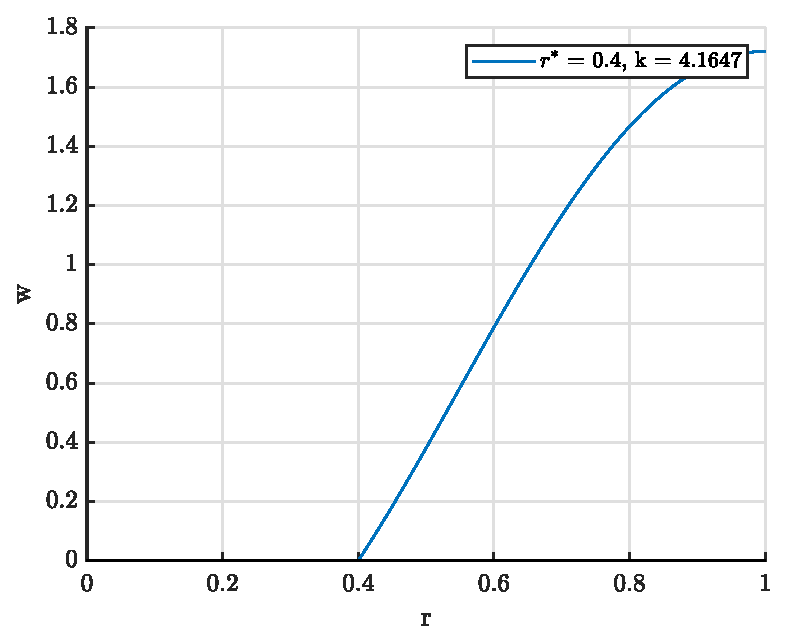
\includegraphics[width=\linewidth]{exampleKRstar}
    \caption{An example solution plot}
    \label{fig:exampleKRstar}
\end{figure}


The set of valid solutions to this problem are those which satisfy the constraint
\[w(r_*) = W + k(AJ_0(kr_*) + BY_0(kr_*)) = 0\]
The plot figure~\ref{fig:contourSolutions} shows the $k,r_*$ combinations which satisfy the constraint. 

Clearly this can only occur for values of $kR > 3.8$. 

The first branch of this (extending from $kR\approx 3.8$) corresponds to natural solutions, whereas further branches give unwanted behaviour, which introduce reversed flow.

Code - homogeneousODE.m


\begin{figure}[h]
    \centering
    \label{fig:contourSolutions}
    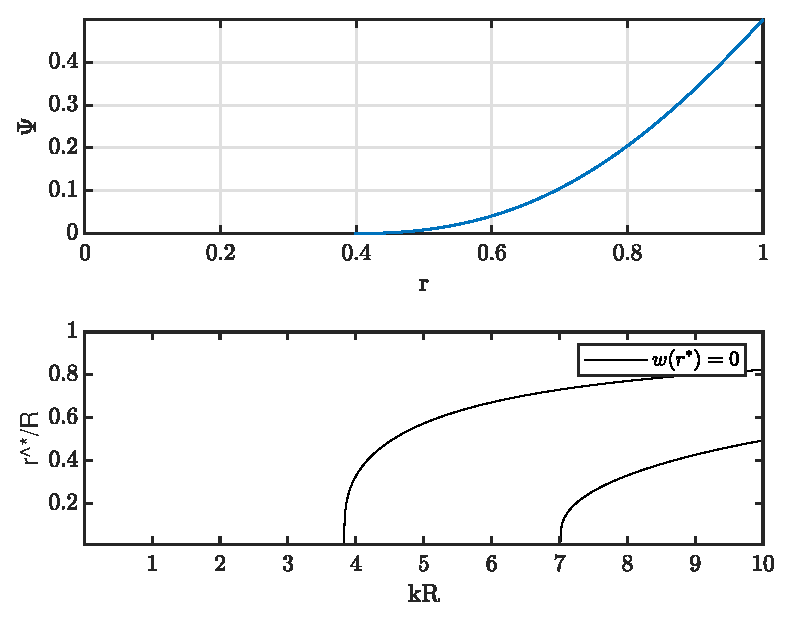
\includegraphics[width=\linewidth]{kRstarContour}
    \caption{Solution set for the simplified problem}
\end{figure}
\newpage


\clearpage



%Tasks:
% \subsection{Lamb-Oseen Vortex}
% The Lamb-Oseen vortex (or Q' vortex)
% \[\ddn \psi z 2 + \ddn \psi r2 - \frac1r \dd\psi r= r^2 \frac{dH}{d\psi} - C\frac{dC}{d\psi}\]

% Q' vortex 
% \[v = \frac{2\pi \Gamma}{r} (1-e^{-r^2/\delta^2})\]
% same $w=W$.
% \begin{align*}
%     C = rv &= r\left(\frac{2\pi \Gamma}{r} (1-e^{-r^2/\delta^2})\right)\\
%      &=2\pi \Gamma (1-e^{-r^2/\delta^2})
% \end{align*}




% %Finite Difference Scheme
% Using forward finite differences:
% \[\dd \psi r(r_0) = \frac{\psi(r_0 +h) - \psi(r_0)}{h} + O(h) \]
% \[\ddn \psi r 2(r_0) = \frac{\psi(r_0+h) - 2\psi(r_0) + \psi(r_0-h)}{h^2} + O(h)\]
% Where $h$ is some small perturbation away from $r_0$.
% Truncate by neglecting the $O(h)$ terms





%https://en.wikipedia.org/wiki/Buckingham_%CF%80_theorem

%rstar to zero is a singular point with a delta function solution
have to assume things for outside of the region for $\Psi$.  I.e. if we go above the maximum input value then some assumption, and if we go below the minimum then it is a stagnation point
%THIS IS IMPORTANT TO MENTION IN THE WRITE UP
%\psi < 0 is a stagnation point

see if we can do it for the wall stagnation zones (i.e. psi goes to 0 near R)
so when $\Psi > \frac12 WR^2$
Plug it into H and C
\[H = (\Omega R)^2 + \frac12 W^2\]
\begin{align*}
    \dd H\psi = 0\\
C = \Omega R^2\\
\dd C\Psi = 0
\end{align*}
Which then yields the separable first order ODE
\[\ddn \Psi r 2 - \frac1r \dd\Psi r = 0 \]
And hence
\begin{align*}
\dd\Psi r = Ar\\
\Psi = \frac12 Ar^2 + B 
\end{align*}


our left hand side could be written as
\[r \dd{}r \left(\frac1r \dd \Psi r\right)\]
using staggered grid 
\[\ddn \Psi r 2 = \frac1r \dd\Psi r\]
 at the boundary r=0


\subsection{Numerics}

Solving the ODE numerically:
\[\ddn \Psi r 2 - \frac1r \dd \Psi r = r^2 \dd H\Psi + C\dd C\Psi\]
finite difference - divide r as a grid of $N$ intervals.
So our grid spaces over $R$, 
\[r_i = \Delta r_i, \quad \Delta  = \frac RN\]
So (check this)
\[\ddn \Psi r 2 = \frac{\Psi_{i+1} - 2 \Psi_i + \Psi_{i-1}}{\Delta ^2}\]
\[\dd \Psi r = \frac{\Psi_{i+1} - \Psi_{i-1}}{2\Delta }\]
\[\Psi_0 = 0, \quad \Psi_N = \frac12 W R^2\]
Which should work for the index $i$ until we reach the bifurcations/stagnations


Should end up with a matrix equation
%[A] \Psi = r sol
\[
\begin{pmatrix}
1 & 0&\hdots &0 & 0 \\
&&\mathbf{A}&&\\
0&0&\hdots & 0 & 1
\end{pmatrix}
\begin{pmatrix}
\Psi_0\\
\mathbf{\Psi}\\
\Psi_N
\end{pmatrix}
=
\begin{pmatrix}
0\\
\mathbf{f}\\
\frac12 W R^2
\end{pmatrix}
\]
A should be the finite difference version of 
\[\ddn \Psi r 2 - \frac1r \dd \Psi r = 0\]
I.e. for the $i^{th}$ row of $\mathbf{A}$
\[A(i) =\frac{A(i+1) - 2*A(i) + A(i-1)}{\Delta ^2} - \frac{A(i+1) - A(i-1)}{2r(i)\Delta } \]
\[A_{ij} =\begin{cases}
1    & j=i=1\\
1/\Delta^2 +1/(2r_i \Delta)& j=i-1\\
2/\Delta^2    & j=i\\
1/\Delta^2 -1/(2r_i \Delta)& j=i+1\\
1   & j=i=N\\
0   & otherwise
\end{cases}\]

For the full equation
\[\ddn\Psi z2 + \ddn\Psi r2 - \frac1r \dd\Psi r + \Psi(\frac{4\Omega^2}{W^2} - \frac1{r^2}) = 0 \]
\[\Psi = \frac12 Wr^2 + rF \]
\[F = \frac{\Psi}{r} - \frac12 Wr\]
Boundary conditions for $F$ relate to those for $\Psi$.
\[\Psi(R) = \frac12 WR^2 \implies F(R) = 0\]
\[\Psi(r_*) = 0 \implies F(r_*) = \frac12 Wr_*^2\]





when we look at the vortex breakdown problem, introduce a coordinate transformation
\[\eta = \frac{r - r_*}{R-r_*}\]
\[\eta = 0, r=r_*, \eta = 1 r=R\]
\[\dd\Psi r = \dd\Psi \eta \dd\eta r = \frac{1}{R-r_*} \dd\Psi \eta\]
\[\ddn \Psi r2 = \frac{1}{(R-r_*)^2} \ddn \Psi \eta 2\]



use the same conditions we have used anyway where $\Psi(r_*) = w(r_*) = 0$
%google potential flow
Rankine body problem:
At some point on the radius $r_0$, we get $v = K/r_0$ for some constant $K$ 
find $K = \Omega r_0^2$?

%then we do q vortex numerically (but not yet)




\subsection{Rankine Body}
$w = W$, 
\[v = \begin{cases}
    \frac{\Gamma}{{2 \pi r}}, &r > r_0 \\
\Omega r ,& r \leq r_0
\end{cases}  \]
Where the second condition was the previous solution. Since the velocity profile is now piecewise defined, the streamfunction must also be, i.e. it is necessary to split the streamfunction into 2 regions to solve this problem. The upstream regions:
 \[\begin{cases}
         \Psi_{inner}, & 0\leq r\leq r_0 \\
         \Psi_{outer}, & r_0\leq r\leq R
     \end{cases}
 \]
%should probs get \Psi = Ar^2 + B in the new region
Note that $r_0$ is defined upstream, so the position of the region may have moved downstream to a new radius, $\hat{r}$, and hence, downstream, these regions will become around $\hat{r}$ instead of $r_0$. We enforce some similar conditions as to the normal problem:
\begin{align*}
    \Psi(r_*) &= 0, \\
    \Psi(R) &= \frac12 WR^2,\\
    w(r_*) &= 0
\end{align*}
With the added condition that $\Psi$ must remain continuous around $\hat{r}$
I.e.
\[\lim_{r^-\to \hat{r}} \Psi(r^-) = \lim_{r^+ \to \hat{r}} \Psi(r^+)\]
And
\[\lim_{r^- \to \hat{r}} v(r^-) = \lim_{r^+ \to \hat{r}} v(r^+)\]
Where $\Psi(r^-)$ is $\Psi$ defined for $r \leq \hat{r}$ and $\Psi(r^+)$ is defined in the region $r \geq \hat{r}$.

The region for $\Psi(r)$ with $r\in [0,r_0]$ will be the same as before, i.e.
\[\Psi(r) = \frac12 Wr^2 + r(AJ_1(kr) + BY_1(kr))\]

For the region $r_0<r<R$ the problem must be resolved from the SL equation
\[\ddn \Psi r 2 - \frac1r \dd\Psi r = r^2 \frac{dH}{d\Psi} - C \frac{dC}{d\Psi}\]
\[C = rv = \frac{\Gamma}{2\pi}\]
\[\frac{dC}{d\Psi} = 0\]
\begin{align*}
    H &= \frac12 (u^2 + v^2 + w^2) + \frac{p}{\rho}\\
    &= \frac12 (0 + \frac{\Gamma^2}{4\pi^2 r^2} + W^2) + \int \frac{C^2}{r^3} dr\\
    &=   \frac12 (\frac{\Gamma^2}{4\pi^2 r^2} + W^2) + \int \frac{\Gamma^2}{4 \pi^2r^3} dr\\
    &=   \frac12 (\frac{\Gamma^2}{4\pi^2 r^2} + W^2) -\frac{\Gamma^2}{8 \pi^2r^2} \\
    &= \frac{W^2}{2}\\
    \frac{dH}{d\Psi} &= 0
\end{align*}

And hence the SL equation gives
\begin{align*}
 \ddn \Psi r 2 - \frac1r \dd\Psi r &= r^2 \frac{dH}{d\Psi} - C \frac{dC}{d\Psi}\\
 \ddn \Psi r 2 - \frac1r \dd\Psi r &= r^2 \frac{dH}{d\Psi} - C \frac{dC}{d\Psi}\\
\ddn \Psi r 2 - \frac1r \dd\Psi r &=0\\
\end{align*}

Which results in:
\[\Psi = Cr^2 + D, \quad r \geq \hat{r}\]
\[w = \frac1r \dd\Psi r = 2C\]
With the requirement that there is no discontinuity at $\hat{r}$, i.e.
\[\Psi = \frac12 W\hat{r}^2 + \hat{r}\left(AJ_1(k \hat{r}) + BY_1(k\hat{r})\right) = C\hat{r}^2 + D\]
And using the same for $w$
\[w(\hat{r}) = W + k(AJ_0(k\hat{r}) + BY_0(k\hat{r})) = 2C\]
And lastly the wall condition
\[\Psi(R) = \frac12 W R^2 = C\hat{r}^2 +D\]

With
\[w(r_*) = 0\]
\[\frac{\Gamma}{2\pi r_0} = \Omega r_0 \implies \Omega = \frac{\Gamma}{2\pi r_0^2} \]
\[k_{outer} = \frac{2\Gamma}{2\pi W r_0^2} = \frac{\Gamma}{\pi W r_0^2}  \]
Noting that the values for $A$ and $B$ are obtained from the $r_*$ condition.



%can use \mathrm{} or \text{} for roman subscripts
The coefficients for $\Psi$ have to be resolved, since the condition $\Psi_{inner}(R) = \frac12 WR^2$ cannot be imposed.\\

Parameters
\[r_0,\hat{r}, r_*, R,k, \Gamma, W, A,B,C,D\]
We can fix $r_0$, $R$, $k$, $W$ and $\Gamma$.
This is $11$ parameters, where $5$ are fixed. Require $6$ conditions.
%%%
%%%Instead of explaining them in the itemize, i should explain them prior, and have footnotes
%%%
Impose:

\renewcommand{\theenumi}{\arabic{enumi})}    
\begin{enumerate}
    \item \label{rankine::1}$w(r_*) = 0$ (as before)
    \item \label{rankine::2} $\Psi_{inner}(r_*) = 0$ (as before)
    \item\label{rankine::3} Since at the wall $\Psi$ must remain the same, this applies to where $v$ is changed, i.e. $\Psi_{inner}(\hat{r}) = \frac12 W r_0^2$ 
    \item\label{rankine::4} For continuity, $\Psi_{outer}(\hat{r}) = \frac12 W r_0^2$ 
    \item\label{rankine::5} $w_{outer}(\hat{r}) = w_{inner}(\hat{r})$\\
    \item\label{rankine::6} $\Psi_{outer}(R) = \frac12 WR^2$ 
\end{enumerate}


Redo the problem instead getting $A,B$ from~\ref{rankine::2} and~\ref{rankine::3}

\[\Psi_{inner}(r_*) = 0\]
\[\Psi_{inner}(\hat{r}) = \frac12 W r_0^2\]




Use this for $A,B$
\begin{align*}
    \Psi_{inner}(r_*) &= \frac12 Wr_*^2 +r_*(AJ_1(kr_*) + BY_1(kr_*)) =0\\
    &=r_*(AJ_1(kr_*) + BY_1(kr_*)) =-\frac12 Wr_*^2\\
    \Psi_{inner}(\hat{r}) &= \frac12 W\hat{r}^2  +\hat{r}(AJ_1(k\hat{r}) + BY_1(k\hat{r})) =\frac12 W r_0^2\\
    &=\hat{r}(AJ_1(k\hat{r}) + BY_1(k\hat{r})) =\frac12 W (r_0^2 - \hat{r}^2)
\end{align*}

This gives the matrix system for $A,B$ below. Note that the system relies on the unknowns $r_*$ and $\hat{r}$.
\[\begin{pmatrix}
    r_*J_1(kr_*) & r_*Y_1(kr_*)\\
    \hat{r} J_1(k\hat{r}) & \hat{r} Y_1(k\hat{r})
\end{pmatrix}
\begin{pmatrix}
    A\\B
\end{pmatrix} = \begin{pmatrix}
    - \frac12 Wr_*^2\\
    \frac12 W (r_0^2 - \hat{r}^2)
\end{pmatrix}\]


\[
\begin{pmatrix}
    A\\B
\end{pmatrix} = \frac{1}{det}\begin{pmatrix}
     \hat{r} Y_1(k\hat{r})& -r_*Y_1(kr_*)\\
    -\hat{r} J_1(k\hat{r}) & r_*J_1(kr_*)\\
\end{pmatrix}\begin{pmatrix}
    - \frac12 Wr_*^2\\
    \frac12 W (r_0^2 - \hat{r}^2)
\end{pmatrix}\]

\begin{align*}
    A &= \frac{1}{\det} \left(\hat{r} Y_1(k\hat{r})\left(-\frac12 Wr_*^2\right) - r_*Y_1(kr_*) \left(\frac12 W(r_0^2 - \hat{r}^2)\right)\right)\\
    B &= \frac{1}{\det} \left(-\hat{r}J_1\left(-\frac12 Wr_*^2\right) + r_*J_1(kr_*) \left(\frac12 W(r_0^2 - \hat{r}^2)\right)\right)
\end{align*}

Where

\begin{align*}
\det &= \hat{r}r_* Y_1(k\hat{r})J_1(kr_*) - \hat{r}r_* J_1(k\hat{r}) Y_1(kr_*)\\
&= \hat{r}r_*\left(Y_1(k\hat{r})J_1(kr_*) -  J_1(k\hat{r}) Y_1(kr_*)\right)
\end{align*}

This for $r_*$
\begin{align*}
    w_{inner}(r_*) = W + k(AJ_0(kr_*) + BY_0(kr_*)) =0
\end{align*}

Get $C$ from:
\begin{align*}
    w_{outer}(\hat{r}) = w_{inner}(\hat{r})\\
    2C = W + k(AJ_0(k\hat{r}) + BY_0(k\hat{r}))\\
    C = \frac12\left(W + k(AJ_0(k\hat{r}) + BY_0(k\hat{r}))\right)
\end{align*}

Get $D$ here:
\begin{align*}
    \Psi_{outer}(R) = CR^2 + D = \frac12 WR^2\\
    D = \frac12 WR^2 - C
\end{align*}

%this for \hat{r}
Hence get $\hat{r}$ from 
\begin{align*}
    \Psi_{outer}(\hat{r}) = C\hat{r}^2 + D = \frac12 Wr_0^2\\
    C\hat{r}^2 + \frac12 WR^2 -C = \frac12 Wr_0^2\\
    \left(\frac12\left(W + k(AJ_0(k\hat{r}) + BY_0(k\hat{r}))\right)\right) (\hat{r}^2 - 1) = \frac12W(r_0^2 - R^2)\\
    \left(AJ_0(k\hat{r}) + BY_0(k\hat{r})\right)(\hat{r}^2 - 1) =\frac1{k}W(r_0^2 - R^2 -1)\\
\end{align*}




For physically valid solutions, we must impose the condition of no net change on the momentum from upstream to downstream  on the momentum (Escudier, Keller). The momentum is defined as
\[s = 2\pi \int_0^{r_t} \left(\rho w^2 + p\right) rdr\]
%$r_a = r_*$, $r_b = \hat{r}$, $r_c = r_0$, and $r_t = R$.
Which comes to:
\[\Delta s = \frac{\pi}{4} \rho U^2 k^2 r_c^2 \left[-r_b^2 + \frac14 \left(\frac{r_b^4 - r_a^4}{r_c^2}\right) + \frac34 r_c^2 + \frac12 r_c^2 \log \left(\frac{r_b^2}{r_c^2}\right)\right] = 0\]




\begin{figure}[h]
    \centering
    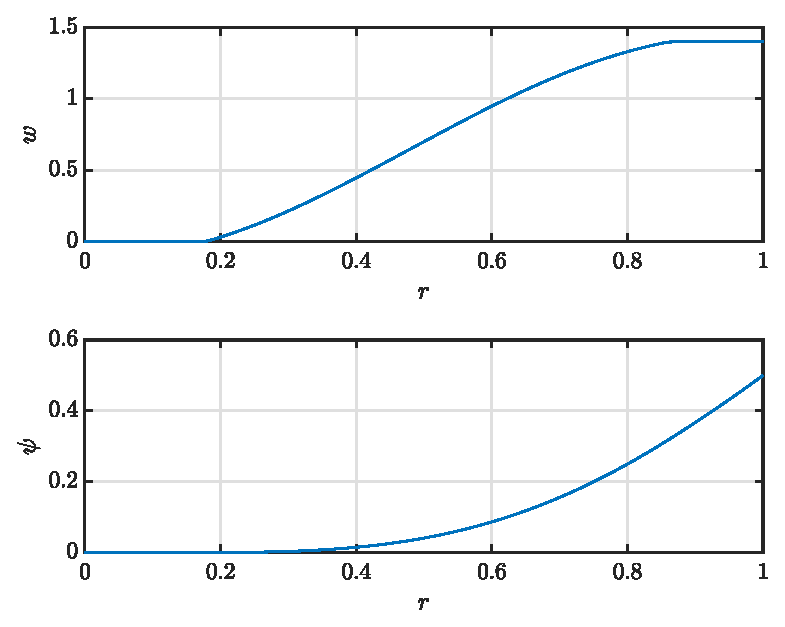
\includegraphics[width=\linewidth]{rankineExample.eps}
    \caption{A solution of $w$ and $\Psi$ for the Rankine problem with $0$ net momentum, $k = 3.8961, r_0 = 0.8619, r_* = 0.1784$. Obtained using }
    \label{fig:rankineExample}
\end{figure}



\begin{figure}[h]
    \centering
    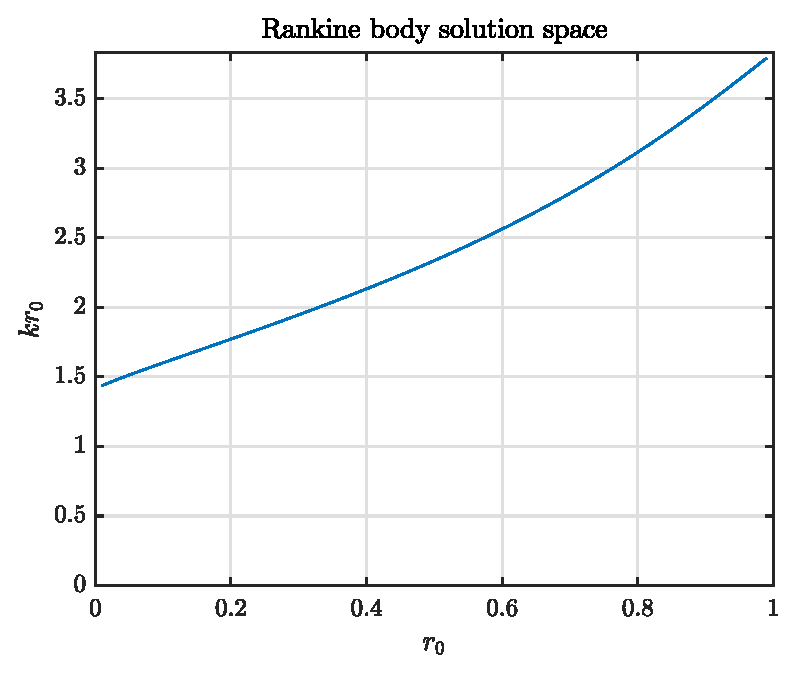
\includegraphics[width=\linewidth]{rankineSolutionSet.eps}
    \caption{Solution space for the Rankine body problem}
    \label{fig:rankineSolutions}
\end{figure}

Figure~\ref{fig:rankineSolutions} shows the solution set for the problem. It displays the same results as those found in (Escudier, Keller), with the same asymptote $kr_0 \to \sqrt{2}$ as $r_0 \to 0$. The results in the two figures come from \verb|rhatrstarmomentum.m| and \verb|numericalSolutionSetRankine.m| respectively
%%%
%put the plot on the document 
%summarise the papers that connect these and show relationships between them with this work (even just some paragraphs and plots)
%

%start on Burgers vortex
%

%%%
\subsection{Lamb-Oseen Vortex}
%pretty sure this is the Lamb-Oseen vortex but trent called it burgers
Q-vortex without a Jet.
Start with 
\[w = W\]
\[v = \frac{\Gamma}{2\pi r} \left(1 - e^{-r^2/\delta^2}\right)\]
\[\frac{d^2\Psi}{dr^2} - \frac1r \odd \Psi r = r^2 \odd H\Psi - C \odd C\Psi \]
Solve from $r_*$ to $R$ numerically.

Generate grid from $r_*$ to $R$.

Boundary conditions as normal
\[\Psi(R) = \frac12 WR^2\]
\[\Psi(r_*) = 0\]
\[w(r_*) = 0\]
And the standard upstream flow 
\[\Psi(r)  =\frac12 Wr^2\]
Non-dimensional parameter may be something like $\frac{\Gamma}{WR}$ (we can probably relate this to $kr_0$ for the rankine problem)



Eventually do the same thing as before with $s$ and $\Delta s$.
\[s = \int_0^R \left(\rho w^2 + p\right) rdr = \int_0^{r_*} p(r_*) rdr + \int_{r_*}^R \left(\rho w^2 + p\right) rdr\]
Use
\[\frac1\rho \dd p r = \frac{v^2}{r} = \frac{\Gamma^2}{4\pi^2r^3+}\left(1-e^{-r^2/\delta^2}\right)^2\]
\[\Psi = \frac12 W r^2 \implies r = \sqrt{\frac{2\Psi}{W}}\]
\begin{align*}
    C &= rv = \frac{\Gamma}{2\pi} \left(1-e^{-r^2/\delta^2}\right)\\
    \dd C\Psi &=\frac{\Gamma}{2\pi} \dd{}\Psi \left(1-e^{-r^2/\delta^2}\right)\\
    &=\frac{-\Gamma}{2\pi} \dd{}\Psi \left(e^{-r^2/\delta^2}\right)\\
    &=\frac{-\Gamma}{2\pi} \dd{}\Psi \left(e^{-2\Psi/W\delta^2}\right)\\
    &=\frac{\Gamma}{W\delta^2\pi} \left(e^{-2\Psi/W\delta^2}\right)\\
    &=\frac{\Gamma}{W\pi\delta^2} e^{-r^2/\delta^2}
\end{align*}
\begin{align*}
    \odd H\Psi &= \odd H r \odd r\Psi \\
    &=\odd r\Psi \odd{}r\left(\frac12 \left(u^2+v^2 + w^2\right) + \frac{p}{\rho}\right)\\
    &=\frac{1}{\sqrt{2W\psi}} \odd{}r\left(\frac12 v^2 + \int\frac{C^2}{r^3}dr \right)\\
    &=\frac{1}{Wr} \left(\frac12 \odd{v^2}r + \frac{v^2}{r} \right)\\
    &=\frac{1}{Wr} \left(\frac{\Gamma^2}{4r\pi^2} \left(\frac{-1}{r^2} +2e^{-r^2/\delta^2}\left(\frac{1}{r^2} + \frac{1}{\delta^2}\right) -e^{-2r^2/\delta^2} \left(\frac{1}{r^2} + \frac{2}{ \delta^2}\right)\right) +  \frac{\Gamma^2}{4r\pi^2}\left(\frac{1 - 2e^{-r^2/\delta^2} + e^{-2r^2/\delta^2}}{r^2}\right) \right)\\
    &=\frac{\Gamma^2}{4Wr^2 \pi^2} \left(2e^{-r^2/\delta^2}\left(\frac{1}{r^2} + \frac{1}{\delta^2}\right) -e^{-2r^2/\delta^2} \left(\frac{1}{r^2} + \frac{2}{ \delta^2}\right) +\frac{ - 2e^{-r^2/\delta^2} + e^{-2r^2/\delta^2}}{r^2}\right)\\
    &= \frac{\Gamma^2}{2Wr^2\delta^2\pi^2} \left(e^{-r^2/\delta^2} - e^{-2r^2/\delta^2}\right)\\
    &= \frac{\Gamma^2}{4\Psi\delta^2\pi^2} \left(e^{-2\Psi/W\delta^2} - e^{-4\Psi/W\delta^2}\right)\\
\end{align*}

How I got the middle term:
\begin{align*}
    \odd{v^2}{r} &= \odd{}r \left(\frac{\Gamma}{2\pi r} \left(1-e^{-r^2/\delta^2}\right)\right)^2\\
    &= \frac{\Gamma^2}{4\pi^2} \odd{}{r} \left(\frac{1 - 2e^{-r^2/\delta^2} + e^{-2r^2/\delta^2}}{r^2}\right)\\
    &= \frac{\Gamma^2}{4\pi^2} \left(\frac{-2}{r^3} -2\left(-\frac{2e^{-r^2/\delta^2}}{r^3} - \frac{2e^{-r^2/\delta^2}}{r\delta^2}\right) + \left(-\frac{2e^{-2r^2/\delta^2}}{r^3} - \frac{4e^{-2r^2/\delta^2}}{r \delta^2}\right)\right)\\
    &= \frac{\Gamma^2}{2r\pi^2} \left(\frac{-1}{r^2} +2e^{-r^2/\delta^2}\left(\frac{1}{r^2} + \frac{1}{\delta^2}\right) -e^{-2r^2/\delta^2} \left(\frac{1}{r^2} + \frac{2}{ \delta^2}\right)\right)
\end{align*}


% \begin{align*}
%     \ddn\Psi r2 - \frac1r \dd\Psi r &=  r^2 \odd H\Psi - C \odd C\Psi\\
%     &=\frac{\Gamma^2}{2W\delta^2\pi^2} \left(e^{-r^2/\delta^2} - e^{-2r^2/\delta^2}\right) - \frac{\Gamma}{2\pi} \left(1-e^{-r^2/\delta^2}\right)\frac{\Gamma}{W\pi\delta^2} e^{-r^2/\delta^2}\\
%     &= \frac{\Gamma^2}{2W \delta^2 \pi^2} \left(e^{-r^2/\delta^2} - e^{-2r^2/\delta^2} - \left(e^{-r^2/\delta^2}-e^{-2r^2/\delta^2}\right)\right) \\
%     &= 0
% \end{align*}
\begin{align*}
    \ddn\Psi r2 - \frac1r \dd\Psi r &=  r^2 \odd H\Psi - C \odd C\Psi\\
    &=\frac{r^2\Gamma^2}{4\Psi\delta^2\pi^2} \left(e^{-2\Psi/W\delta^2} - e^{-4\Psi/W\delta^2}\right) - \left(\frac{\Gamma}{2\pi} \left(1-e^{-2\Psi/W\delta^2}\right)\right)\left(\frac{\Gamma}{W\delta^2\pi} \left(e^{-2\Psi/W\delta^2}\right)\right)\\
    &=\frac{r^2\Gamma^2}{4\Psi\delta^2\pi^2} \left(e^{-2\Psi/W\delta^2} - e^{-4\Psi/W\delta^2}\right) - \frac{\Gamma^2}{2W\delta^2\pi^2}\left(1-e^{-2\Psi/W\delta^2}\right) \left(e^{-2\Psi/W\delta^2}\right)\\
    &= \frac{\Gamma^2}{2W\delta^2\pi^2}\left(\frac{r^2W}{2\Psi} \left(e^{-2\Psi/W\delta^2} - e^{-4\Psi/W\delta^2}\right) -\left(e^{-2\Psi/W\delta^2}-e^{-4\Psi/W\delta^2}\right)\right)\\
    \ddn\Psi r2 - \frac1r \dd\Psi r &=  \frac{\Gamma^2}{2W\delta^2\pi^2}\left(\left(\frac{r^2W}{2\Psi} - 1\right) \left(e^{-2\Psi/W\delta^2} - e^{-4\Psi/W\delta^2}\right) \right)\\
\end{align*}
Giving the system
\begin{align*}
    \Psi_1 ' &= \Psi_2\\
    \Psi_2' &= \frac1r \Psi_2 + \frac{\Gamma^2}{2W\delta^2\pi^2}\left(\left(\frac{r^2W}{2\Psi_1} - 1\right) \left(e^{-2\Psi_1/W\delta^2} - e^{-4\Psi_1/W\delta^2}\right) \right)\\
\end{align*}

Take limit as $\Psi\to0$ in matlab and use that in some suff area.

Could use bvp5c and break it into a system of first order odes.


So if we change the boundaries - using a `Linear Lagrange interpolating polynomial'
So that the end points are fixed.
\[\eta = \frac{r-r_*}{R-r_*}\]
\begin{align*}
    r-r_* = \eta(R-r_*)\\
    r = \eta(R-r_*) + r_*   
\end{align*}


Such that $\eta \in [0,1]$.
In the function we can get $r$ from $\eta$ 

For finite differences we can just use a newton iteration, or use something like fsolve.



I SHOULD PLOT DOWNSTREAM $v$ for all our equations also



To use the $r_*$ and $w$ parts, we can use $w = \frac1r\dd\Psi r $


Try putting in the homogeneous solution to the solver to see if it works (i.e. the one with $v = \Omega r$ and $w=W$).

We should expect that the Lamb-Oseen vortex should be a more smooth version of the Rankine problem - so we should be able to compare the two.

May want to find $v_{max} = r_0$ to compare to the previous problem.
Should expect the circulation goes to $\Gamma / 2 \pi$ as $r\to \infty$.




Of course we have to have
\[\lim_{r\to 0} \frac1r \dd\Psi r < \infty\]
So use l'hopital's rule
\[\lim_{r\to 0} \frac1r \dd\Psi r = \ddn\Psi r2\]
But we know $\psi = 0$ at $r=0$ ( so we can ignore this )



So we will just use
\[\ddn \Psi r2 |_i - \frac1r \dd\Psi r|_i = f(r_i,\Psi_i)\]
With 
\[\Psi_1 = 0\]
And
\[\Psi_n = \frac12 WR^2\]

We will have 1 based indexing 
Alternatively 
get the derivatives at the mid points
\[\dd\Psi r\pipe_{i+1/2} = \frac{\Psi_{i+1} - \Psi_i}{h_r}\]
Where $h_r$ is the step.





Alternatively


Can rewrite the left hand side as

\[r\left(\dd{}r \left(\frac1r \dd\Psi r\right)\right)\]
And plug in the last thing
\[\]









% Hence
% \[\Psi(r) = ar^2 + b\]






When we do finite differences, grab a computational variable (call it $\eta$ for now)
\[ \eta = \frac{r - r_*}{R-r_*}\]
So now we are computing in $0<\eta<1$.
So try plugging it into the ODE:
\[d\eta = \frac{dr}{R-r_*}\]
\[\dd\Psi r = \dd\Psi\eta \dd\eta r = \frac{1}{R-r_*} \dd\Psi\eta\]

If we don't know $r_*$ the $\eta$ vector becomes
\[\begin{pmatrix}
    \eta_0\\
    \vdots\\
    \eta_{N-1}\\
    r_*
\end{pmatrix}\]
This will be a non-linear problem so we will need to solve using \verb|fsolve|.

To get guesses could use rankine vortex stuff - 

For a linear flow we could use
We know that $\psi(r_*) = 0$ and $\psi(R) = \frac12 WR^2$. We could guess that $\psi$ is constant, $\psi = Ar^2 + B$.

Try plotting $w(r_*)$ for various $r_*$ to help find guesses (require it to be $0$)



If using $\eta$, the ODE becomes
$\psi(\eta = 0) = 0$ and $\psi(\eta=1) = \frac12 WR^2$

\[\dd \Psi r = \frac{1}{R-r_*} \dd\Psi\eta \]
\[\ddn\Psi r 2 = \frac{1}{(R-r_*)^2}\ddn\Psi\eta 2\]
\[r = \eta(R-r_*)) +r_*\]
DE becomes
\[\frac{1}{(R-r_*)^2}\ddn{\Psi}\eta2  -\frac{1}{\eta(R-r_*)) +r_*} \frac1{R-r_*}\dd\Psi \eta =0\]
\[\frac{1}{R-r_*}\ddn{\Psi}\eta2  -\frac{1}{\eta(R-r_*)) +r_*}\dd\Psi \eta =0\]



\clearpage
Write a function which calculates the residual, i.e.
\[\hat{r}_i = LHS - RHS| _i\]
and then fsolve on that

Send through the vector
\[\begin{pmatrix}
    \Psi_1\\
    \vdots\\
    \Psi_N\\
    r_*
\end{pmatrix}\]



Might be worth looking at setting the RHS
\[r^2 \odd H\Psi + C \odd C\Psi \]
As a function $f(r,\Psi)$ and the settings
\[f(r,\Psi) = \begin{cases}
    \ldots, &\text{ if } 0 \leq \Psi \leq \frac12 WR^2\\
    0 & otherwise
\end{cases}\]

\clearpage
%trent said - 
% Not sure what I was thinking here. For vector f divergence theorem is

% int d f_i/ d x_i dV = int f_i n_i dS

% Put f_i = p c_i, where c_i is a component of constant vector. Then

% int c_i (d p / d x_i) dV = int c_i p n_i dS

% => c_i (int d p / d x_i dV - int p n_i dS) = 0 for any c_i

% => int d p / d x_i dV = int p n_i dS

% I think that's better.



% The equation for $s$ comes from the Euler equations
% (Don't need to use this / know this - we did it with tensors)
% gives
% \[\dd{u_iu_j}{x_i} = -\frac1\rho \dd p{x_i}\]
% \[\int_v \dd{u_iu_j}{x_i} +\frac1\rho \dd p{x_i} dv\]
% Use divergence theorem 
% \[\int \nabla \cdot v dv = \int v\cdot \hat{n} ds\]
% \[\int_v \dd{u_iu_j}{x_i} +\frac1\rho \dd p{x_i} dv = \int_s \dd{u_iu_j n_i}{x_i} +\frac1\rho \dd p{x_i} ds\]

% \[v_i = p \delta_{ij}, \quad p\delta_{ij}n_i = pn_j\]
% \[=\int_s u_iu_j n_i + \frac p \rho n_j ds\]
% Since we are considering a cylinder, we get $0$ along the boundary of the cylinder, and so we only care about the inlet and outlet.
% At the inlet the normal faces in the negative $w$
% \[u_in_i = -w\]
% \[u_in_i = w\]
% \[\int_{(1)} -w^2 -\frac{p}{\rho} dS + \int_{(2)} \int w^2  +\frac{p}{\rho} dS =0 \]
% Which is literally in flux = out flux. 



%%%%
%%
%% 
For the method - since we're stuck
try using
\[r\dd{}r \left(\frac1r \dd \Psi r\right) = r\frac{\frac1r \dd\Psi r|_{i+\frac12} - \frac1r \dd{\Psi}{r}|_{i-\frac12}}{\Delta r}\]
Where $r_{i+1/2} = \frac{r_i + r_{i+2}}{\Delta r}$ and $\dd\Psi r |_{i+\frac12} = \frac{\Psi_{i+1} - \Psi_i}{\Delta r}$

and using the rusak method, by letting $y = r^2/2$

We may have to make our own solver, or use an available one ().

Wang and rusak the dynamics of a swirling flow in a pipe and transitions to axisymmetric vortex breakdown

do some research on numerical solutions of axisymmetric swirling flow 



Trent had a book with a means of numerically solving the system, which will work in 2D as well
\[\ddn \Psi z 2 + \ddn \Psi r2 - \frac1r \dd \Psi r = - r \eta\]

We are given an $\eta$. 
If we let $\Psi_{i,j} = \Psi(r = r_i, z = z_j)$
\[\ddn \Psi z2\pipe_{i,j} = \frac{\Psi_{i,j+1} - 2 \Psi_{i,j} + \Psi_{i,j-1}}{\Delta z^2}\]

\[\ddn \Psi r2\pipe_{i,j} = \frac{\Psi_{i+1,j} - 2 \Psi_{i,j} + \Psi_{i-1,j}}{\Delta r^2}\]

\[\dd \Psi r \pipe_{i,j} = \frac{\Psi_{i+1,j} - \Psi_{i-1,j}}{2 \Delta r}\]

\begin{align*}
    \frac{\Psi_{i,j+1} - 2 \Psi_{i,j} + \Psi_{i,j-1}}{\Delta z^2} + \frac{\Psi_{i+1,j} - 2 \Psi_{i,j} + \Psi_{i-1,j}}{\Delta r^2} - \frac1{r_i} \left( \frac{\Psi_{i+1,j} - \Psi_{i-1,j}}{2 \Delta r}\right) = - r_i \eta_{i,j}
\end{align*}
Could write $r_{i,j}$ in case it changes in $j$.

Of course to write this as a linear system, we have to get form $A\vec \Psi = b $
So we would have to write the vector $\Psi$ as 
\[\begin{pmatrix}
    \Psi_{1,1}\\
    \Psi_{2,1}\\
    \vdots\\
    \Psi_{m,1}\\
    \Psi_{1,2}\\
    \vdots\\
    \Psi_{1,n}\\
    \vdots\\
    \Psi_{m,n}
\end{pmatrix}\]

So the index of $\Psi_{i,j}$ will be $i + m(j-1)$ let $v_{i+m(j-1)} = \Psi_{i,j}$, and also expanding $\eta$ in this fashion.
Hence the vector $\vec v$ is
\[\begin{pmatrix}
    v_1\\
    v_2\\
    \vdots\\
    v_{mn}
\end{pmatrix}\]
Then the system becomes, after an index shift:
\begin{align*}
    \frac{v_{i+m(j+1)} - 2 v_{i+m(j)} + v_{i+m(j-1)}}{\Delta z^2} + \frac{v_{i+1+m(j)} - 2 v_{i+m(j)} + v_{i-1+m(j)}}{\Delta r^2}\\
     - \frac1{r_i} \left( \frac{v_{i+1+m(j)} - v_{i-1+m(j)}}{2 \Delta r}\right) = - r_i \eta_{i+m(j)}\\
\end{align*}

% \begin{align*}
%     \frac{v_{i+m(j)} - 2 v_{i+m(j-1)} + v_{i+m(j-2)}}{\Delta z^2} + \frac{v_{i+1+m(j-1)} - 2 v_{i+m(j-1)} + v_{i-1+m(j-1)}}{\Delta r^2}\\
%      - \frac1{r_i} \left( \frac{v_{i+1+m(j-1)} - v_{i-1+m(j-1)}}{2 \Delta r}\right) = - r_i \eta_{i+m(j-1)}\\
% \end{align*}
% \begin{align*}
%         v_{i-1+m(j-1)}\left(\frac{1}{\Delta r^2} + \frac{1}{2\Delta r r_i}\right) + v_{i+m(j-1)} \left(-\frac{2}{\Delta z^2} - \frac{2}{\Delta r^2}\right) + v_{i+1+m(j-1)} \left(\frac{1}{\Delta r^2} - \frac{1}{2\Delta r r_i}\right)\\
%         + v_{i+m(j-2)} \left(\frac{1}{\Delta z^2}\right) + v_{i+m(j-1)}\left(\frac{1}{\Delta z^2}\right) = -r_i \eta_{i+m(j-1)}
% \end{align*}
\begin{align*}
        v_{i-1+m(j)}\left(\frac{1}{\Delta r^2} + \frac{1}{2\Delta r r_i}\right) + v_{i+m(j)} \left(-\frac{2}{\Delta z^2} - \frac{2}{\Delta r^2}\right) + v_{i+1+m(j)} \left(\frac{1}{\Delta r^2} - \frac{1}{2\Delta r r_i}\right)\\
        + v_{i+m(j-1)} \left(\frac{1}{\Delta z^2}\right) + v_{i+m(j+1)}\left(\frac{1}{\Delta z^2}\right) = -r_i \eta_{i+m(j)}
\end{align*}
Ignoring the boundary conditions on $\Psi(0,z), \Psi(r,0), \Psi(R,z), \Psi(r,Z)$
\[A_{a,b} = \begin{cases}
    \frac{1}{\Delta r^2} + \frac{1}{2\Delta r r_i}  & b = a - 1 \\
    -\frac{2}{\Delta z^2} - \frac{2}{\Delta r^2}    & b = a \\
    \frac{1}{\Delta r^2} - \frac{1}{2\Delta r r_i}  & b = a + 1 \\
    \frac{1}{\Delta z^2}                            & b = a - m \\
    \frac{1}{\Delta z^2}                            & b = a + m 
\end{cases}\]

See if I can construct $A$. especially with sparse.
With boundaries $\Psi(r=0) = 0$, $\Psi(z=0) = f(r)$, $\Psi(r=R) = f(R)$ and $\Psi(z=Z) = ???$

Wang, Rusak use $\dd\Psi z = 0$. And at the right boundary it might make sense to use a backwards difference so we don't have to deal with the $n+1$.
So that $\Psi_{i,j}$ is stored in index 


for the time solver precompute the LU factorisation of the matrix.

\clearpage
\subsection{Outer vortex breakdown}
Considering the initial problem for vortex breakdown, except perhaps the breakdown is a pocket expanding from $R$ rather than $0$. I.e. the breakdown occurs about the wall rather than the center.
So assuming $r^\dagger $ is our outer vortex breakdown radius


This simply means obtaining a new $A$, $B$ and $k$.
\[\Psi(r) = \frac12 W r^2 + r(A J_1(kr) + BY_1(kr))\]
\[w(r) = W + k(A J_0(kr) + B Y_0(kr))\]
Such that
\[w(r^\dagger) = 0,\qquad \Psi(0) = 0,\quad and \quad \Psi(r^\dagger) = 0  \]
 
To enforce $\Psi(0) = 0$ note that $\lim_{r\to 0} \frac{Y_1(kr)}{r} = -\infty$. Hence it is necessary to set $B = 0$. 
\[\Psi(r) = \frac12 Wr^2 + rAJ_1(kr), \quad w (r) = W + kAJ_0(kr)\]
And to enforce 
$\Psi(r^\dagger) = 0$
\[\implies Ar^\dagger J_1(kr^\dagger) = -\frac12 Wr^{\dagger2}\]
\[A = \frac{-Wr^{\dagger}}{2J_1(kr^\dagger)}\]
And obtain $k$ using
\[w(r^\dagger) = 0\]
\[k AJ_0(kr) = -W\]


\[\Psi(r^\dagger) = \Psi(R) = \frac12 WR^2\]








%%%TRY SOLVING THE REGULAR PROBLEM WITH r^* = 0 and B = 0

%%%summary of project
%%%Vortex breakdown states
%Columnar flows
%- rotating flows DONE
% - analytics DONE
% - numerics DONE
%- rankine vortex DONE
%   analytics DONE
%   numerics DONE
%- Burgers vortex DONE
%   analytics DONE
%   numerics DONE
%- Q' vortex
%   numerics
%Pipe flow
%-finite length (straight) pipe
%-pipe with sink outlet (apparently theres a paper on this that i should find)
%-tornados?
%-variable radius


\clearpage
\section{Appendix}
\subsection{Supplementary Materials}
This is where all the basic fluid mechanics knowledge should be (definitions, etc.)

\subsection{Resources}
Books:
An Introduction to Fluid Dynamics
Batchelor

Swirling flow states in finite-length diverging or contracting circular pipes
Zvi Rusak


Wall-separation and vortex-breakdown zones in a solid-body rotation flow in a rotating finite-length straight circular pipe
Zvi Rusak, and Shixiao Wang

The Navier-Stokes equations: a classification of flows and exact solutions
Drazin, Riley


%looking for r_* = 0 and w(r_*) = 0
%go through analytics to find this

\end{document}
